\documentclass{report}
\usepackage{graphicx}
\usepackage[utf8]{inputenc}
\usepackage[fontsize=15pt]{fontsize}

\title{\textbf{ME5010 : Logistic Map}}

\begin{document}
\author{Shyam Sridhar\\ Nitesh Singh \\ Rudramuni TS \\ Pavan Kumar \\ Aman Gautam }
\maketitle

\section{Introduction}

\begin{center}$x_{n+1} = rx_n(1-x_n)$\end{center}
Logistic Equation is primarily know for modeling population growth of animals and it is part \textbf{Chaos Theory}, which is branch of mathematics that demonstrates how deterministic mathematical system could lead to unpredictability.

Logistic equation is characterized by it's sensitivity to input parameters. Very small changes in $x_0$ and $r$ could lead to drastic changes in predictions, and thus leading to Chaos. Due to this particular nature logistic map was once used to generate array of seemingly unrelated numbers also called pseudo-random number. It could generate unpredictability from deterministic machine. Beside that it is also used in cryptography for encryption of data where encrypted data would be very sensitive to the key i.e small variation in key would not decrypt/decode the encrypted data allowing only one and one unique key to decrypt the data.

In this project our aim is to explore behaviour of logistic map. It's sensitivity to initial parameters, period doubling, unpredictability and device a pseudo-random number generator (PRNG). We will use same PRNG to encrypt an image.



\newpage
\section{Logistic Equation}

The following equation also called logistic equation is used to model population growth.
\begin{equation}
x_{n+1} = rx_n(1-x_n)
\end{equation}
where:

$x_n$ = population in $n$th generation,

$r$ = growth rate

\begin{figure}[!h]
    \centering
    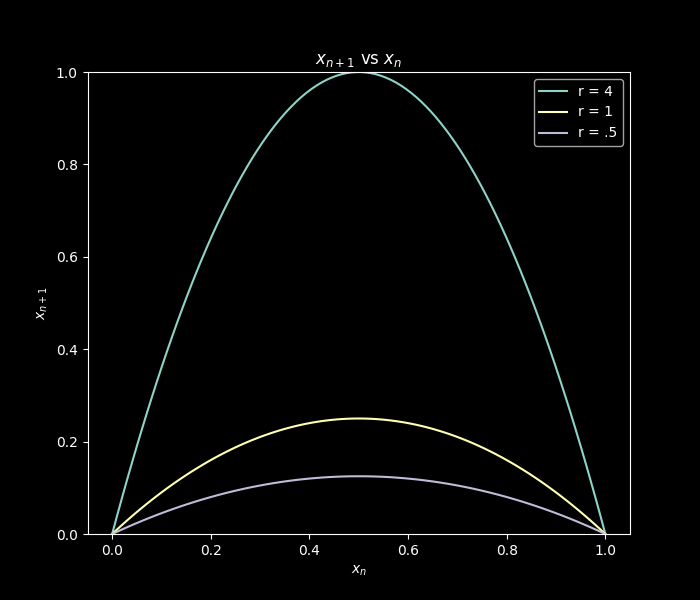
\includegraphics[scale=.5]{images/xnvsnp1.png}
    \caption{$x_{n+1}$ vs $x_n$ (Such functions are also called single humped functions)}
    \label{fig:my_label}
\end{figure}

For $r \in [0, 4]$ the function $x_{n+1}$ maps the closed interval [0, 1] into itself. We shall
restrict our attention to these values of r. Also we'll see r is the main factor contributing to unpredictability of equation.

As observed from the graph below $x_{n}$ is not exactly predictable for every r.




\begin{figure}[!h]
    \centering
    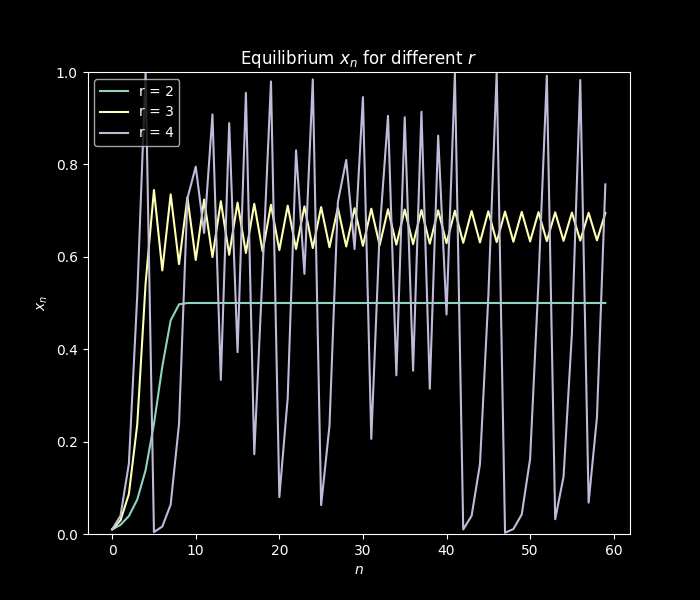
\includegraphics[scale=.4]{images/eqfordifr.png}
    \caption{$x_n$ at equilibrium for different r's}
    \label{fig:my_label2}
\end{figure}

On varying r and plotting equilibrium $x_{n}$ we get the following observations.

\begin{itemize}
  \item $r < 3$ One Equilibrium position of x is seen.
  \item $r > 3$ Two Equilibrium position of x is seen.
  \item As r is increased further we have multiple equilibrium positions
\end{itemize}

\textbf{Fixed Points} \\



Equation can be said to be converging when

$x_{n+1} \to x_n$

Thus, we can write

$x = rx(1-x)$

From above equation we get the following solutions or equilibrium points.\\

$x = 0$ and $x = 1 - \frac{1}{r}$\\

For $r \in [0,1)$ $x = 0$ acts as attractor (solution converges to this point)

For $r \in 1$ $x = 0$ acts as repellor (x seems to diverge from x = 0 line)

And $x = 1 - \frac{1}{r}$ is an attractor for $1 < r < 3$ and a repeller for $r > 3$.\\

This can be obtained from the slope of $f_r = rx(1-x)$ at x, that is equal to $r(1-2x)$ for points 0 and $1-\frac{1}{r}$.\\

$f'_r(0) = r$ , $f'_r(1-\frac{1}{r}) = 2-r$\\



Slope less than 1 implies $x_n$ will be attracted to the solution and vica-versa. Observe there is no attractors for $r>3$ thus explaining why there is no particular solution in that case.
\end{document}

